\documentclass{article}
\usepackage[final]{nips_2018}
\usepackage[utf8]{inputenc}
\usepackage[T1]{fontenc}
\usepackage{hyperref}
\usepackage{url}
\usepackage{booktabs}
\usepackage{amsfonts}
\usepackage{amsmath}
\usepackage{nicefrac}
\usepackage{microtype}
\usepackage{gensymb}
\usepackage{graphicx}
\usepackage{subfig}
\usepackage{wrapfig}
\usepackage{hyperref}

\title{Fully Autonomous Grasping Using Vision}
\author{George Maratos\\\\Advisor: Dr. Brian Ziebart\\\\Secondary Commitee Member: Dr. Xinhua Zhang}

\begin{document}
\maketitle

\newpage
\begin{abstract}
Fully autonomous grasping is a planning task. A machine senses objects in its
environment, and predicts the configuration of its end effector so that it can
grasp the object. A grasp here is defined as a stable envelopement, by the machine's
end effector, so that it can manipulate the object for simple tasks like picking
and placing. When considering a fully autonomous setting, where the machine has no
external help, grasping can be divided into three separate tasks. First the machine
must be able to detect that an object is present in its field of view, then it must
detect a location on the object which is most suitable for grasping, and finally
it must position its end effector so that it can successfully execute the grasp.

In this project, I explore these three areas of fully autonomous grasping where the
machine's only sensing capabilities are 2-D images from a camera. I design an
architecture which can learn how to find grasps on the image plane, and train it
on the Cornell Grasping Dataset. Given the difficulty of the task and the
small size of the dataset, I employ techniques to extend the utility of the
limited data like pretraining and image augmentations. I also explore the task
of object detection on the Cornell Dataset. The tasks described above are
difficult, and since there is already work that successfully solves the task
in certain settings, I investigate if the task can still be solved
using a lower complexity model. A lower complexity would be beneficial because
most state of the art models, as far as I know, have very large architectures
that require large amounts of computing power or a GPU to solve in reasonable time.

\end{abstract}

\newpage
\tableofcontents
\newpage
\section{Introduction}
In the robotic grasping problem the goal is, given an object, select a grasp
configuration such that the object can be restrained and
manipulated to some desirable end. Finding such configurations is difficult
because of the multi-modal nature of the input and the fact that there can be
more than one suitable grasping location, which means the machine must choose
one grasp from many optimal ones to attempt.
Some of the earliest reviews of algorithms for grasping \cite{shimoga96,bicchi00},
shows that the premliminary work involved solving unconstrained linear programming
problems using objectives that measure dexterity and grasp quality. A grasp
algorithm in this context is one that is able to calculate the stability or
equilibrium of its grasp, and they are collectively refered too in the
review as \textit{robot grasp synthesis algorithms}.

The review by Sahbani \textit{et al.} \cite{sahbani12}, makes a distinction
between methods that model the kinematics and dynamics of a grasp, like the
synthesis algorithms, and methods that mimic human grasp strategies or learn
from data. The former called the analytic methods and the latter empirical.
They divide the analytical techniques into force closure methods and task
oriented. The authors determine that force closure is able to find stable
grasps but are usually not task oriented, and the task oriented strategies tend
to be computationally intensive. The empirical methods on the other hand can
model task oriented features, but struggle to generalize well to new objects.

Bohg \textit{et al.} \cite{bohg14} observe that grasping methods typically aim
to address the following object types: fully known, familiar, or fully unknown.
When considering the empirical methods, fully known represents objects that
have been seen in the training data before and the grasping problem reduces to
locating the object and applying a similar grasp to those from experience.
The familiar objects are assumed to have some matching characteristics to objects
from the training data, like shape, color, and texture. Familiar objects
introduce a new challenge of calculating similarity between objects so that
the appropriate grasp can be determined. On the other hand, grasping algorithms
will have no experience to utilize when approaching fully unknown objects. Methods
of this category typically rely on finding structures in the features to
synthesize a grasp.

The focus of this work is to build empirical models for grasp synthesis using
the Cornell Grasp Datset \cite{lenz15}, and evaluating them on familiar and
fully unknown objects. Section 2 will describe previous methods for grasp
synthesis. Section 3 will focus on analysis of the dataset and a description
of the task. Section 4 will contain the experimental section. Finally, Section
5 is the conclusion and future works.

\section{Existing Grasp Synthesis Methods}
\subsection{Analytical Methods}
The earliest mention of qualities of a successful grasp, to the author's
knowledge, is from \textit{Kinematics of Machinery} by Franz Reuleaux
\cite{reuleaux76}.
In it, constant forces are applied to an object and it is considered
constrained if sensible external forces can be balanced. When the
object is in equilibrium, which occurs if the above conditions are
met, then force closure occurs. Nguyen \textit{et al.} \cite{nguyen86},
explored the notion of force closure and developed algorithms for computing
the set of all force closure grasps on simple shapes.
This work is extended by Ferrari \textit{et al.} \cite{ferrari92}, to calculate
a grasp quality criteria. The criteria is measured as the ratio between the force
applied externally and by the fingers. The best grasp is determined by solving
an optimization problem that minimizes the finger force but still can maintain
force closure against a large external force.

Due to the multimodal nature of the task, it could be useful to model various
features of the object being grasped. In the work by Zhang \textit{et al.}
\cite{zhang12}, the authors explore bayesian filtering in $G-SL(AM)^2$. They
build probabilistic models that model various features: the shape of the,
object, mass, and friction coefficient for example. The application of this
is for when you have input data blackout, which could occur if the arm
during operation occludes the visual sensors.

The simulation software \textit{GraspIt!} \cite{miller04}, was developed with
the goal of aiding research in robotic grasping. It has a wide set of features
such as, many different types of hand models, collision detection, and grasp
quality evaluation. It could be used in setting where expensive robotic hardware
is unavailable or used in an algorithm that evaluates grasps in the simulation
before choosing the best one for a physical robot.
The software was applied in work done by Miller
\textit{et al.} \cite{miller03}, where they designed a grasp planning algorithm
that modeled objects as shape primitives and generated poses based off the
primitives.

\subsection{Empirical Methods}
The empirical methods involve techniques that implement learning algorithms that
model the grasping problem from data. This section will only discuss the
non-deep learning methods, deep learning is discussed in another section.

The simulator Graspit! \cite{miller04} enabled researchers to collect synthetic
data for grasping, one example is by Pelossof \textit{et al.} \cite{pelossof04}.
The authors generated synthetic data by subsampling the parameters from
generated grasps and they trained an
SVM-RBF regressor with the goal of predicting grasp quality. They generated
grasps by fixing certain joints, for example to guarantee the palm runs
parallel with the surface of the object, and allowing others to be sampled
randomly within a range. Using their procedure, the authors were able to
generate a dataset with approximately $80\%$ of the grasps having a non-zero
graspability score. Graspability being calculated in the same way as previous
works \cite{ferrari92}.

Robots that are predicting grasps will not always have a complete model of the
input, for example visual sensors might not be able to view an object from all
directions. Kamon \textit{et al.} \cite{kamon96} attempt to predict
grasps from only 2-D images of the object. They solve two problems
simultaneously: choosing grasping points, and predicting the quality of a grasp.
About 2000 grasping examples were collected, which were used for prediction during
testing. Features are extracted directly from the image, for example center of
mass, and were used to calculate the quality of a grasp. The authors claim
that grasp quality can be predicted reliably using only local features.

In some settings, a full 3-d model of the object to be grasped will be unavailable.
The work by Saxena \textit{et al.} \cite{saxena07,saxena08} address this.
Given a set of images of the object in 2-d, it is possible to infer the location of it
in 3-d. Their
approach invovles modeling the probability that a grasp is present in the center of an
image patch. Using synthetic data, they learn a set of parameters via MLE using
logistic regression. The features are extracted from the image set and correspond to
the following: edge filtering, texture masking, and color masking. To predict a grasp
a MAP estimate is calculated for selecting the most probable grasp. In preceeding work
\cite{saxena08a}, they address the issue that predicting a "grasp point" does little to
model the physical limitations of the robotic grasping platform. They further incorporate
depth maps and generate a new set of features that account for other properties:
quatities representing the envelopement of the object by the hand, quantities that
represent the distribution of the mass of the object in relation to the hand, and
quantities that roughly calculate the shape of the object and the alignment of the hand
in relation to this shape. In extending their previous work, their solution is
two-fold with a model for predicting the location of a grasp and another model for
predicting the probability that the robotic arm will be able to achieve the grasp using
the extra features as predictors.

Learning a grasping point in the image plane may be easier for learning algorithms
but they do not model the gripper configuration completely. The work by Jiang
\textit{et al.}
\cite{jiang11}, learn a rectangle configuration that can better represent a parallel
gripper plate end effector. A rectangle, in this case, has $5$ parameters which
correspond to the 2-d coordinate of the top left corner of the rectangle, the height
and width, and the angle between the first edge and the x-axis. They define a score
function, which is a linear combination of features, that represents the quality of
a grasp rectangle. The features are calculated from the pixels within the rectangle, and
consist of 17 filters and 5-bin histograms as a set of quick features and a collection of
more advanced non-linear features are used as well when doing the final inference.
SVM's have been used in the past as a way to rank the quality of a grasp \cite{le10},
in this work inference is done in a two step process
with two separate SVM ranking models. The first model ranks using the features that
are easy to compute, and this prunes the space of possible rectangles. The second ranks
the rectangles chosen by the first model. For calculating the rectangles on an angle,
they rotate the image in discrete intervals of $15\degree$ before calculating
the features.

One approach to leveraging empirical data is to apply KNN
similar to previous works \cite{zhang11,ciocarlie14}.
The objects are represented geometrically and a good grasp is modeled based
on the quality of grasps from previous examples in the same coordinate position.
A simple discriminator is used to compute a binary score for a grasp from the
dataset and a new example. It compares the coordinates from both grasps and
returns $0$ if they contain grasps, and returns $1$ if they do
match. Using this metric, they model the probability of a good grasp occuring
at a coordinate by considering the ratio of good grasps and bad grasps in the
set of nearest neighbors.

Some early approaches try to combine visual features with haptic feedback,
\cite{piater02,coelho01}. Finding parameters for high quality models in this
case is done using Expectation Maximization, learning and execution stage
are not separated. Visual
features are used to recommend grasp configurations, and from these configurations
the machine will probe the surface of the object with its end-effector until
a stable grasp is found. This work represents a critical shift where a grasping
algorithm does not explicitly represent objects geometrically but instead
sythensize a grasp from incomplete images and feedback of the object.

Many works try modeling the probability that a grasp lies in some coordinate
in the image plane. Another approach is to consider grasp synthesis as a
planning problem, which can be about finding a configuration for the machine
in environments of high uncertainty. Sensors could
give a partial view of the object, for example the front of cup, and the machine
must be able to quantify this uncertainty and act based off this information.
A machine that can recognize the uncertainty in a grasp can decide if it has
enough information to attempt the grasp or if it needs to probe the environment
for further data. In Hisiao \textit{et al.} \cite{hsiao07}, the authors
partition the configuration space of the robot into a discrete set of commands
which act as states in a Partially Observable Markov Decision Process.

\subsection{Deep Learning Methods}
The Deep learning methods can be considered a subset of the empirical methods
that has shown promise for many computer vision tasks, see the review
by Voulodimos \textit{et al.} \cite{voulodimos18} for an overview of recent
advances. As described above, some approaches to grasp synthesis involve the
usage of visual features. One challenge in tasks of computer vision is the
selection of powerful and discriminative features, and deep learning methods
are useful for learning features from the data as opposed to hand-crafted ones.

Using the configuration in \cite{jiang11}, where the grasp is represented as
a rectangle, the task can be formulated in two ways.
The first where the machine is asked to evaluate if a given rectangle contains
a grasp, which is known as recognition. The other is detection, where the
machine is asked to identify all possible grasps from an image. The work by
Lenz \textit{et al.} \cite{lenz15}, demonstrated an approach to grasp
detection which involved a two step cascaded approach. First, they employ
a shallow network to learn features that will discriminate good grasp locations
from bad. The network is shallow so that fast detection can occur. Then, they
use a deeper network for selecting the best grasp from the set of grasps
proposed by the first network.

In the work done by \cite{zhou18, zhang18}, the authors design a real-time method
for predicting poses of a parallel gripper plate on RGB and RGB-D images. The extend
the idea
of anchor boxes, mostly used in object detection, and add anchors not just for the
position in an image but also the angle orientation of the rectangle. They design
a network that uses a ResNet50 backbone, and apply a small convolutional filter to
the features for grasp detection and orientation of the end effector. They also use
the Cornell Dataset and employ similar techniques for image augmentation.

A final approach discussed here is the one by Levine \textit{et al.} \cite{levine2018},
and Pinto \textit{et al.} \cite{pinto2016}. The approach is different than others by
learning how to grasp through trial and error. Through thousands of trials, the
robots in both works were able to devise a strategy for grasping objects. The method
for learning was done via Reinforcement Learning, and the data collection step was
fully autonomatic requiring little human intervention.

\newpage

\begin{figure}
\centering
\subfloat{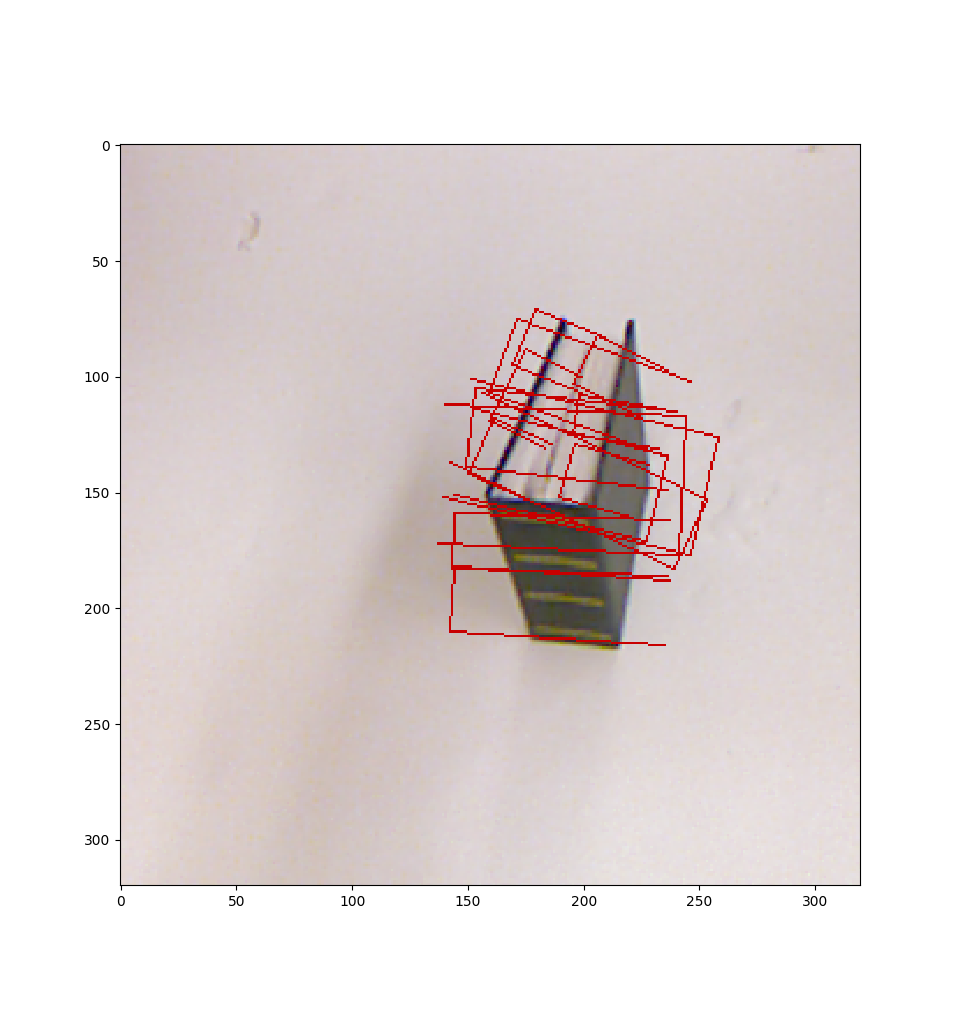
\includegraphics[width=0.3\textwidth]{figures/label_object_norm_1.png}}
\subfloat{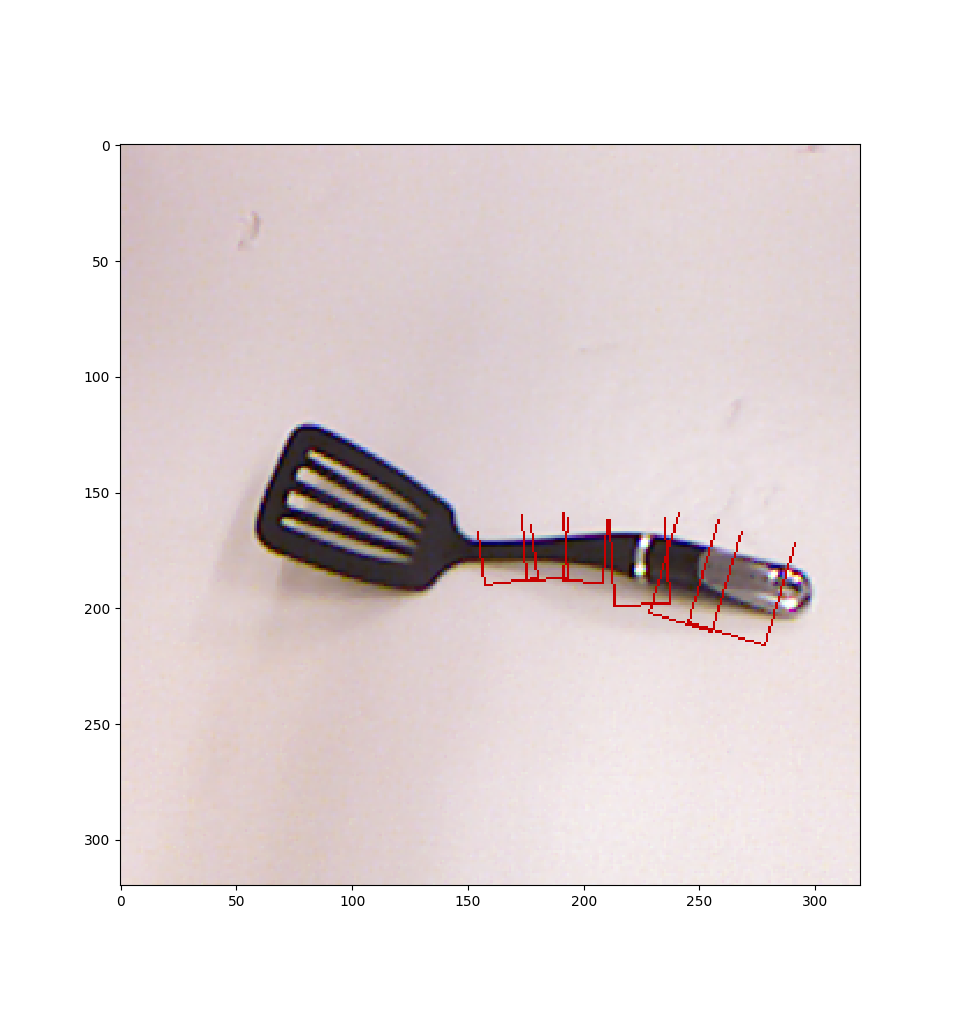
\includegraphics[width=0.3\textwidth]{figures/label_object_norm_2.png}}
\subfloat{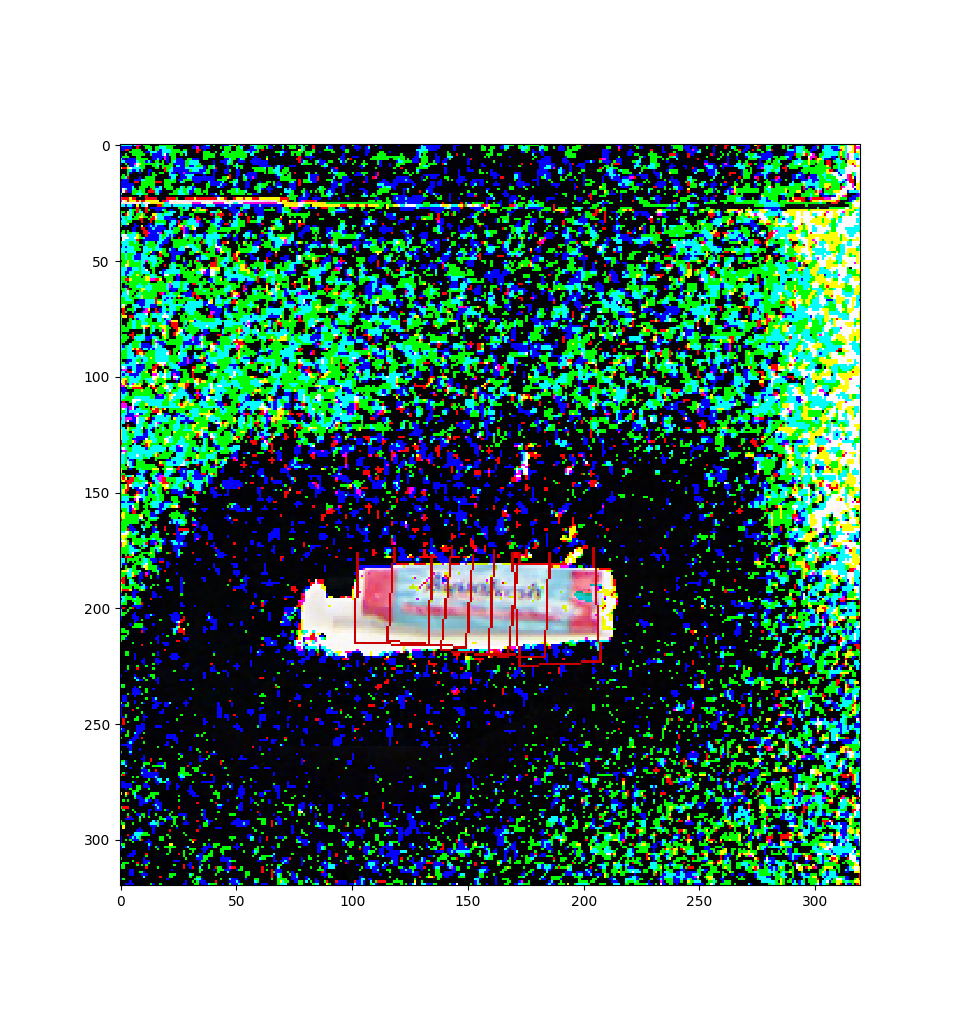
\includegraphics[width=0.3\textwidth]{figures/label_object_norm_3.png}}
\caption{ground truth and images in the dataset, the right most image has background subtraction}
\end{figure}

\section{Data Analysis}
The dataset is approximately 880 images, which contain common
household and office objects. The entire dataset consists of about 10.4 GB.
Each image has one object, centered in the image, placed on a white table.
Every object has a set of grasping rectangles, that are defined by the position
of the corners. Most objects have around 5 rectangles, but there are outliers
with over 20. See the histogram showing the distribution of rectangles per image
in Figure \ref{fig:recdist}.

\begin{wrapfigure}{R}{0.5\textwidth}
\centering
\begin{tabular}{c|c|c|c|}
&Objects&Images&Rectangles\\
\hline
Train&168&617&3567\\
\hline
Val&24&81&456\\
\hline
Test&52&185&1082\\
\hline
Totals&244&883&5105\\
\hline
\end{tabular}
\caption{Summary Counts of the Dataset}
\label{fig:summary}
\end{wrapfigure}

We also observe that the distribution of
the rectangles apears to be normally distributed (see Figure \ref{fig:areas})
and also that width is also normally distributed with length being closer
to a half normal. The other offsets are more uniform.
See Figure \ref{fig:summary} for detailed information about general
information of the dataset.

\begin{figure}
\centering
\subfloat[Old Backgrounds]{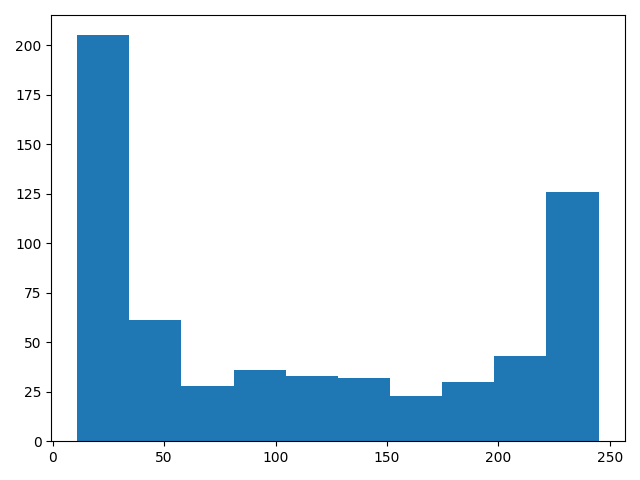
\includegraphics[width=0.4\textwidth]{figures/mean_pixel_dist_train_old_bkg.png}}
\qquad
\subfloat[New Backgrounds]{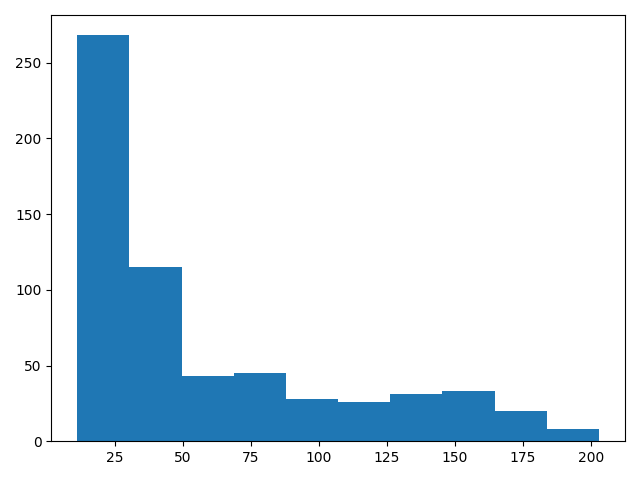
\includegraphics[width=0.4\textwidth]{figures/mean_pixel_dist_train_new_bkg.png}}
\caption{The Change in the Mean Pixel Distribution using the New Backgrounds}
\label{fig:backgrounds}
\end{figure}


The dataset does have a set of labels for classification.
There are $93$ classes in total, with $78$ classes being represented in the
training data.
The classes are more relevant for the object detection task, as the model for
grasping does not learn or use class data explicitly. As such, it will be discussed
more then.

\begin{figure}
\centering
\subfloat[Train]{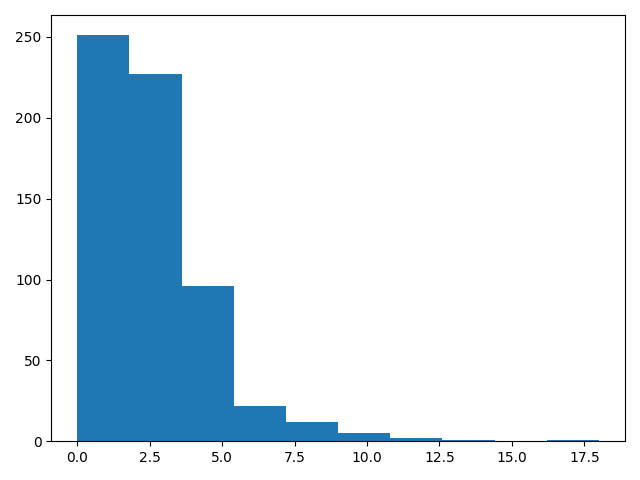
\includegraphics[width=0.4\textwidth]{figures/rec_overlaps_train.png}}
\qquad
\subfloat[Val]{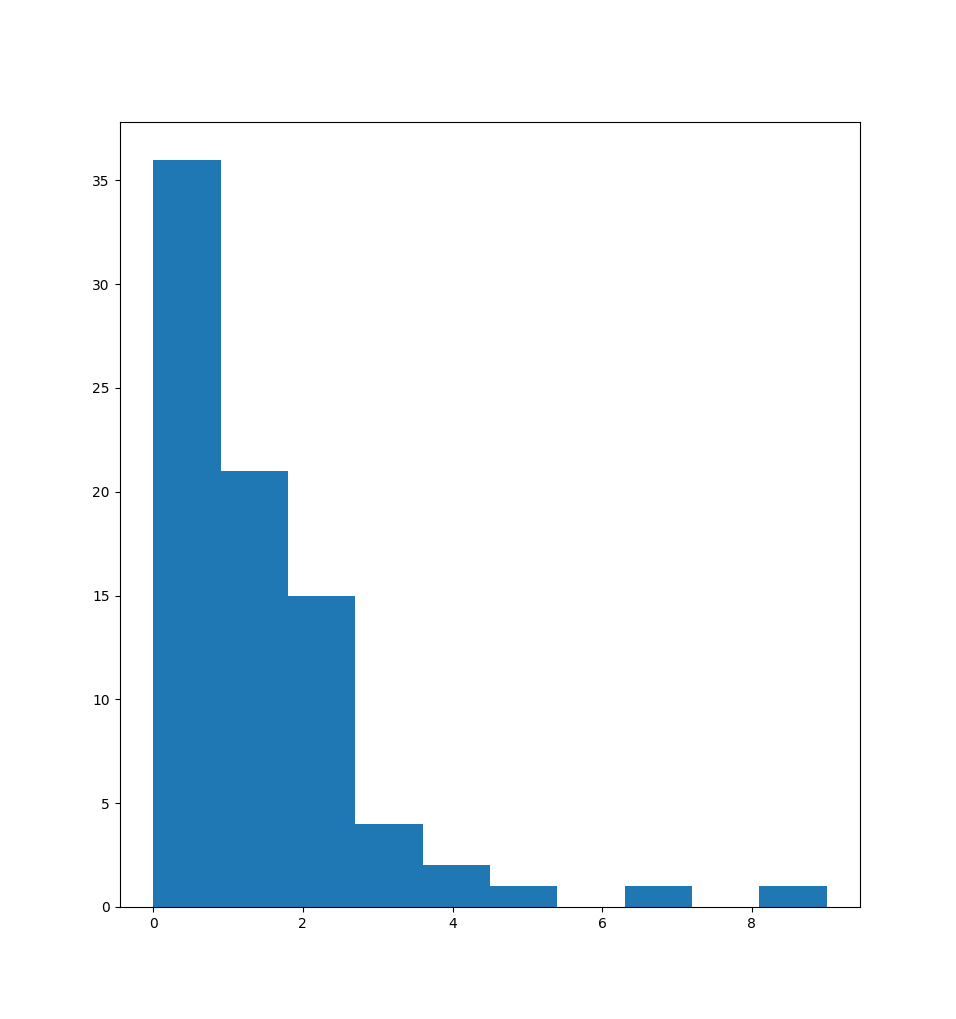
\includegraphics[width=0.4\textwidth]{figures/rec_overlaps_val.png}}
\caption{The Distribution of Number of Overlaps per Image on the Training and Validation Sets}
\label{fig:overlapdist}
\end{figure}

The method used in this paper employs an anchor box
based detection model. The input is divided into a grid of anchors. For each of
these anchors, a prediction is made whether or not a grasp lies inside the
anchor box or not. At the same time, the model predicts where the grasp lies
as an offset of the top left corner of the anchor box. See Figure \ref{fig:example}
for a visual representation of what a prediction looks like.
Selecting the appropriate anchor box width is important, because
since the model makes only one prediction per anchor box there could
be a case where the dataset will have two rectangles that fit in a single
anchorbox.
Here an anchor box is a square with a side length of 32 pixels. This
is chosen because of constraints imposed by the backbone of the network.
See Figure \ref{fig:overlapdist} for a distribution of the number
of overlapping rectangles per image, given that anchor size is 32.

\subsection{Data Preprocessing}
Given that the dataset is small, in comparison with other datasets for deep
learning, it is important to perform data augmentation to prevent overfitting.
Following Zhang \textit{et al.} \cite{zhang18} the augmentation done to each
image is the following, a random flip horizontally, a random flip vertically,
a random rotation of the image about the center ranging from $-30\degree$ to
$30\degree$. The background image is also subtracted to reduce noise. Finally,
the image pixels are normalized to a range of $[0,1]$.

There are cases where the background image subtraction does not fit well with the
original image, and to evaluate the quality we observe the mean pixel value of an
image. As a general rule for evaluating the quality of a subtraction, if an image
has the background removed, then the mean pixel value would be low as the
majority of the pixels have a value of $0$.
If we use the annotations in the dataset, the average
mean pixel value will be approximately $112.11$ when sampled from the training set,
with a standard deviation of $87.62$. Since there could be many mislabels in the
backgrounds, a procedure was developed with searches for the background image that
finds the lowest mean pixel value for each image. Using this method, the mean
drops to $58.51$ with a standard deviation of $49.52$. Since the background images are
virtually the same, being a white table with no object, we hypothesize that there
are some mistakes in the annotations, or that variations in the lighting between shots
have impacted the accuracy of the background images. See Figure \ref{fig:backgrounds} for
details on the shift in mean pixel value.

\begin{figure}
\centering
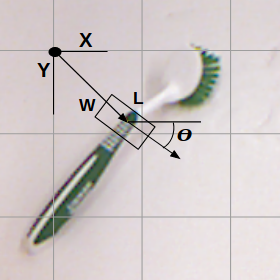
\includegraphics[width=0.3\textwidth]{figures/example_anchor_box.png}
\caption{The image is partitioned into an anchor box grid. If a grasp lies in an anchor box then its position in the box is defined by (X, Y, L, W, and $\theta$)}
\label{fig:example}
\end{figure}

\newpage
\section{Object Detection}
Grasp detection can be seen as a subset of object detection.
As stated earlier, detecting the object to be grasped can be helpful in finding the
optimal grasp location. A proposed approach to grasp detection is to use a standalone
object detection model to filter out background noise, then apply a more expensive
algorithm for detecting grasps and finding end-effector orientation. We explore how
one could apply an object detection module to the Cornell Grasping dataset.

We consider one state of the art model YOLO \cite{redmon16}, which represents a class
of architectures that take a fully convolutional approach to object detection. It has
the advantage over other high performance models like Faster-RCNN \cite{girshick15} of
being faster because there is no region proposal stage. Visual features are convoluted
sequentially and the output of the network is a tensor. The postion of the values in the
tensor are important as they encode information about the location of predictions on the
input image plane.

For our analysis, we use a pretrained model that was trained on MSCOCO \cite{lin14}. Which
is a general purpose, and widely used, dataset for object detection. A question arises of
whether or not MSCOCO will perform well in this setting. If the model
observes many objects that were not present in MSCOCO, its performance might suffer.
We can analyze the precision of the bounding boxes during inference, and how close
the class labels are in both datasets.

Measuring the precision of the bounding boxes is difficult because the Cornell dataset
does not have any annotations for object detection, but we can still get some rough
estimates by understanding
how the data is configured. All images are, for the most part, centered on a white table
and never take up more than roughly a third of the center of the image. So by looking
at the distribution in position of the centers of the bounding boxes and how large the
area of the bounding boxes are we can deduce how well YOLO performs in this new setting.

Starting with examining the class name overlap. YOLO was trained on a set of 81 classes,
and after running a naive search of simply matching names with Cornell we can observe
that there are about seven classes total that have explicit matches.

The distribution of the areas was calculated and shown in Figure \ref{fig:obj_det} a.
What can be observed is a natural split around the bounding box area (square root) of
200. When the examples with areas larger than 200 are filtered out, the total number
of detections is $145$ compared to the original $239$ on the training set. The positions
of the bounding box centers (on the original 320x320 image can be found in Figure
\ref{fig:obj_det} b. The positions are mostly centered, if we consider being centered
as existing in the center $1/3$ of the image. Although, the author admits
that further analysis might be necessary. See Figure \ref{fig:obj_detect} for examples
of detections.

\begin{figure}
\centering
\subfloat[Area Distribution of YOLO Bounding Boxes (square root)]{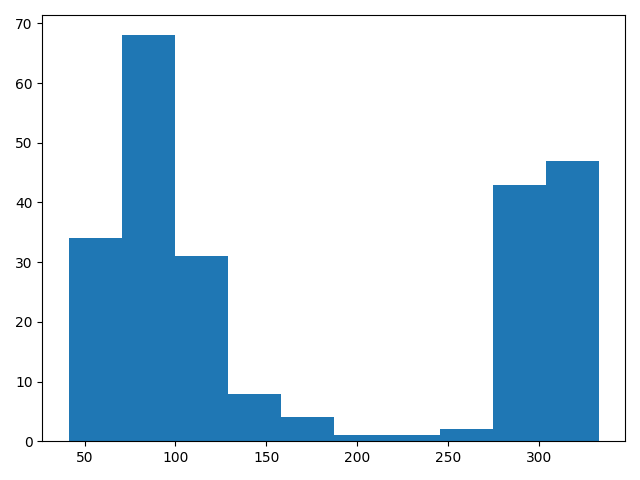
\includegraphics[width=0.3\textwidth]{figures/object_detection_total_areas.png}}
\qquad
\subfloat[Center of Bounding Boxes from Inference with Yolo (filtered)]{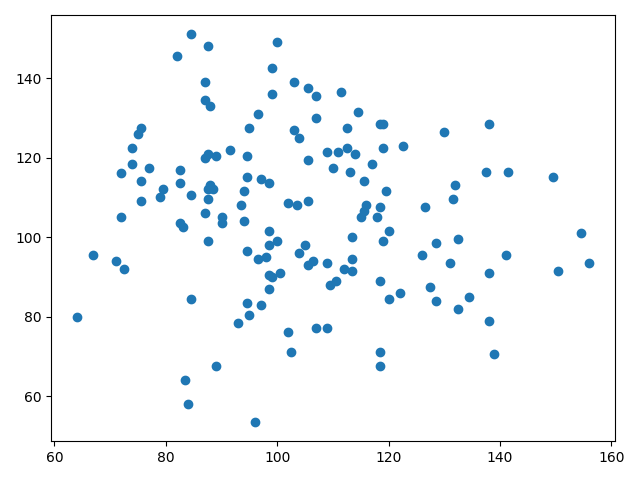
\includegraphics[width=0.3\textwidth]{figures/object_detection_positions_filtered.png}}
\caption{Observations from the Object Detection Experiment}
\label{fig:obj_det}
\end{figure}

\begin{figure}
\centering
\subfloat[Good]{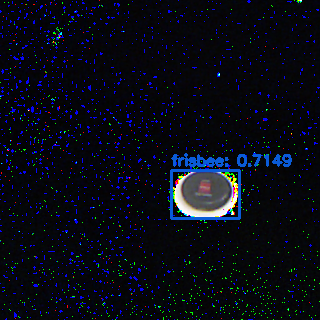
\includegraphics[width=0.2\textwidth]{figures/object_detection_example.png}}
\qquad
\subfloat[Wrong Class]{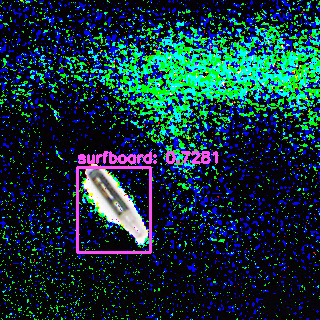
\includegraphics[width=0.2\textwidth]{figures/object_detection_other_example.png}}
\qquad
\subfloat[Bad Precision]{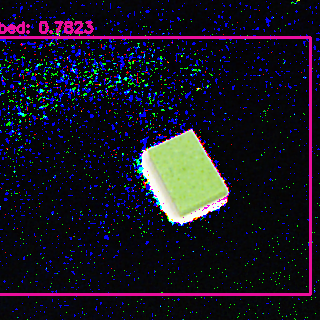
\includegraphics[width=0.2\textwidth]{figures/object_detection_bad_example.png}}
\caption{The Three Examples of Detections When Using YOLO on Cornell}
\label{fig:obj_detect}
\end{figure}

\newpage
\section{Rectangle Grasp Model}
A grasp is defined as a rectangle, oriented in the image plane. A robot with
parallel gripper plates for end effectors would be able to line up its plates
parallel with the short ends of the rectangle (width) and close its gripper along the
long edge (length). This type of end effector can be better understood as a pinching
action.
The grasping model is designed to predict the location of all
the rectangles that would result in a successful grasp. It does this by dividing the
image into a grid of anchor boxes, then makes a prediction for each anchor box. A
prediction involves the detection of a grasp existing in an anchor box, and the five
grasping parameters necessary for configuring the end effector.

See Figure \ref{fig:nn} for a diagram of the architecture.
The model consists of two major parts. The first being the backbone which extracts
visual features from the data, which is VGG16, \cite{simonyan14},
using batch normalization and has approximately 14 million parameters. The
pretraining was done on ImageNet for the task if classification.
The final
piece is a single convolutional layer with seven filters, which represent the
five grasping parameters $x, y, l, w, \theta$ and two scores for graspability.
Figure \ref{fig:example} shows how the five grasping parameters are used to
calculate the location of the grasp. The output of the model is a tensor of
shape (Batch Size) x 7 x (num of Anchors in Width) x (num of Anchors in Height).
During training the ground truths are matched with the corresponding vector of
7 values in the output tensor. To perform inference, the model predicts
whether a not a grasp exists in an anchor by comparing the predicted scores
for graspability and non-graspability
and whenever the graspability score is larger than the non-graspable it
is considered a positive prediction.

The loss function has two components, the first being the binary cross entropy
The cross entropy
represents the loss measure for grasp detection. Detection ground truth, in
this case, is simply $1$ if there exists a grasp and $0$ if it does not.
The grasp configuration loss is calculated by a Smooth L1 Loss between
the predicted 5 values and the calculated ground truth. The total loss is inspired
by the work by Zhang \textit{et al.} \cite{zhang18} who use a similar metric.
The final loss can be calculated as follows.
\begin{equation*}
loss = 2*CrossEntropy(s_p, s_t) + smooth\_l1\_loss(\{t_x, t_y, t_w, t_l, t_\theta\}, \{x_t, y_t, w_t, l_p, \theta_p\})
\end{equation*}

Where $s_p$ is the network's confidence that a grasp exists and $s_t$ is the binary ground
truth.$t_x, t_y, t_w, t_l, t_\theta$ are the predicted configurations and
$x_t, y_t, w_t, l_t, \theta_t$ is the ground truth. Cross entropy is scaled to
emphasize the importance of detection, which is arguably the harder part of the task. The
predicted parameters were encoded the following way. The ground truth is also encoded in
the following format.

\begin{align*}
t_x&=\frac{x-x_a}{w_a} & t_w&=\log(\frac{w}{w_a}) & t_\theta&=\frac{\theta}{2\pi}\\
t_y&=\frac{y-y_a}{l_a} & t_l&=\log(\frac{l}{l_a}) & &
\end{align*}

\begin{figure}
\centering
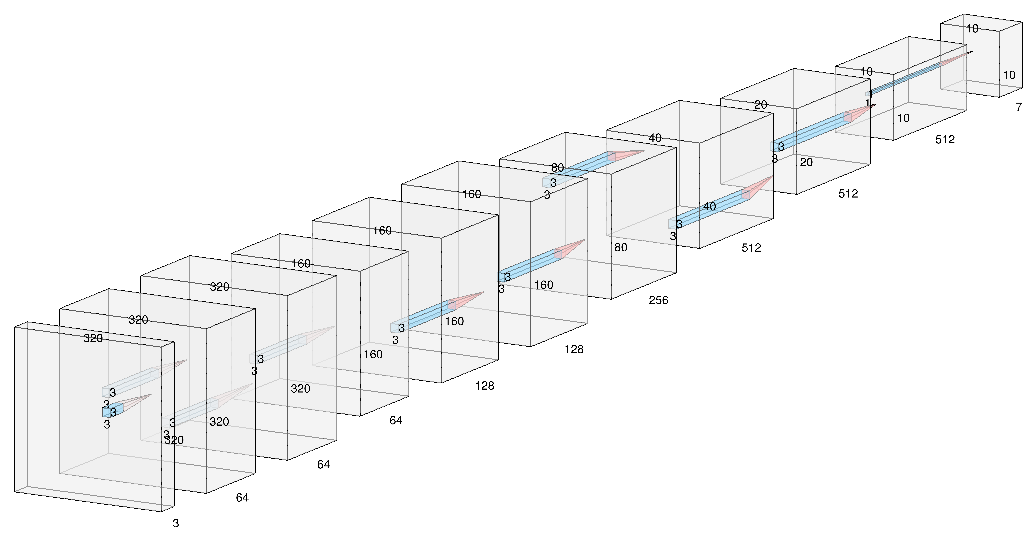
\includegraphics[width=0.4\textwidth]{figures/nn.png}
\caption{Architecture of VGG16 plus head. The predictions are extracted from the final tensor}
\label{fig:nn}
\end{figure}

\newpage
\section{Experiments}

\subsection{Hardware and Software Used}
See Figure \ref{fig:specs} for details about the machine used for training.

\begin{wrapfigure}{R}{0.5\textwidth}
\centering
\begin{tabular}{|c|c|}
\hline
CPU&Intel Xeon E5-2697 @ 2.60 GHz\\
\hline
RAM&157 GB DDR4\\
\hline
GPU&NVIDIA GeForce GTX 1080 Ti 12 GB\\
\hline
\end{tabular}
\caption{Machine Specifications}
\label{fig:specs}
\end{wrapfigure}

All work was done using Python 3, and the major libraries were
Numpy, OpenCv, and Pytorch. Numpy and OpenCV were used for image
processing and augmentation, and all Deep Learning Modules were done
in Pytorch, with GPU support. The pretrained networks also come from
Pytorch, specifically from the torchvision library.
All code and documentation can be found
at \url{https://github.com/gpmaratos/rgrasp.pytorch}. The documentation
is generated using Doxygen.

\subsection{Results}
The prediction space for the Rectangle Grasp Model is very large, there are
$100$ anchors with the majority of them not containing a grasp on average.
This makes training difficult as the model has a tendency to optimize
towards predicting negative for all anchors. There were a couple ways chosen
to mitigate this, the first was to weigh the classes in the cross entropy
calculation in favor of the positive class. In this case, we chose a scale of $1$ to
$\frac{3}{2}$. The next strategy was to use a technique called Hard Mining
\cite{liu15}, which involves sampling specific anchor points instead of
using the whole prediction space. The sampling ratio was $3$ to $1$ in favor of the
negative class. The model's backbone was pretrained on ImageNet as discussed
earlier, but these weights did not remain fixed throughout training and thus
were fine-tuned for the grasping task.

\begin{wrapfigure}{R}{0.5\textwidth}
\centering
\begin{tabular}{|c | c | c | c|}
\hline
&Train&Val&Test\\
\hline
DL&0.256&0.622&0.622\\
\hline
RL&0.11&0.24&0.24\\
\hline
Precision&0.680&0.41&0.38\\
\hline
Recall&0.847&0.37&0.31\\
\hline
F1&0.753&0.38&0.34\\
\hline
Theta&0.014&0.022&0.017\\
\hline
\end{tabular}
\caption{Summary of Rectangle Grasp Model Performance}
\label{fig:test_results}
\end{wrapfigure}

For measuring the performance of the detection, a simple binary metric was
used. Either an anchor did or did not contain a grasp. Precision, recall,
and F1 Score were calculated based on the network's performance using this
metric. Since the network outputs two scores, one for graspability one for
non-graspability, whenever the score for graspability was larger it was
considered a positive prediction for the network. See Figure
\ref{fig:rgrasp_detection} for results on the training and the validation
set for $500$ epochs of training. For results on how the cross entropy
and smooth l1 loss change during training see Figure \ref{fig:rgrasp_loss}.
The test results can be found in Figure \ref{fig:test_results} along with
the final results from the training and validation sets. For examples
of predictions by the model see Figure \ref{fig:rgrasp_examples}.

\begin{figure}
\centering
\subfloat[Precision]{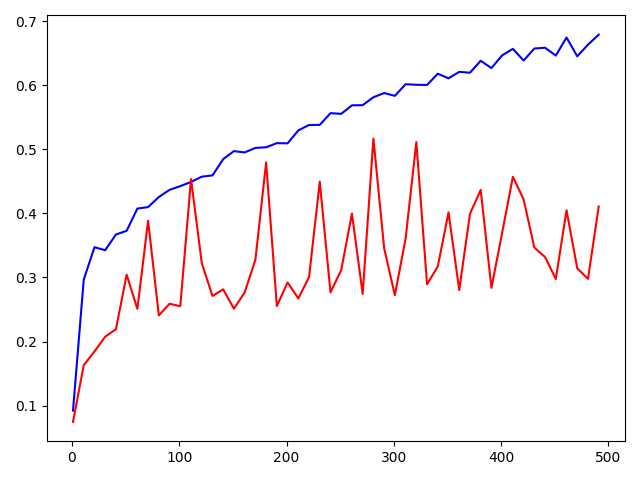
\includegraphics[width=0.4\textwidth]{figures/rgrasp_precision.png}}
\qquad
\subfloat[Recall]{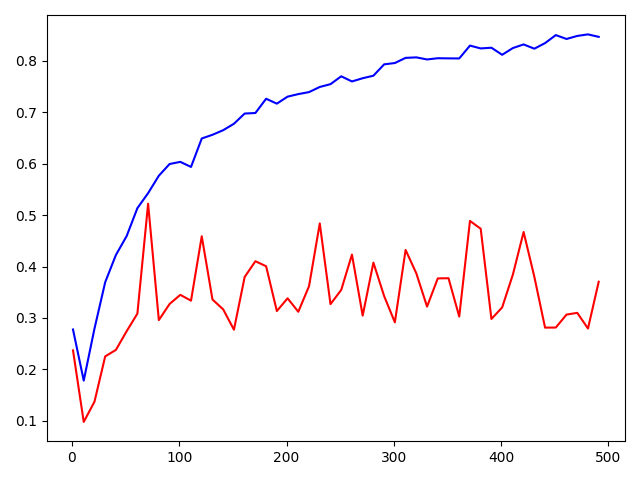
\includegraphics[width=0.4\textwidth]{figures/rgrasp_recall.png}}
\qquad
\subfloat[F1 Score]{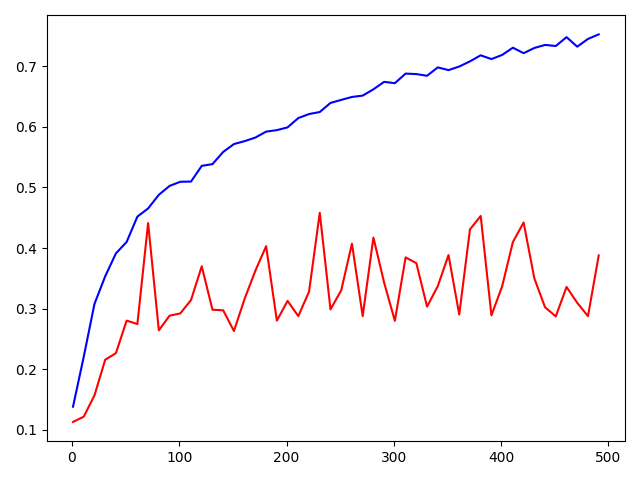
\includegraphics[width=0.4\textwidth]{figures/rgrasp_f1.png}}
\caption{Metrics on Grasp Detection for the Rectangle Grasp Model over 500 Epochs for Train (blue) and Val (red)}
\label{fig:rgrasp_detection}
\end{figure}

\subsection{Conclusion}
An explanation for why the peformance is poor (besides the overfitting
that is clearly occuring after epoch 100) on detection, might be because
the performance metric might be too strict. In most object detection settings,
and in \cite{zhou18, zhang18}, measuring the intersection over union of the
bounding boxes is used. This is because in many cases, the model might predict
a box that encapsulates most of the object but is missing a small portion. In
this scenario the metric used here would consider that incorrect because it
does not overlap completely. It is also worth noting the performance of the
regressor on selecting the angles for orienting the rectangle. By observing
the angle score (represented as theta in the figure) which is one component of
the smooth l1 loss, we can see that on the test set the predicted angle was off
by on average $3\degree$.

Because of the configuration of the network, the features for the detection
and regression component are shared. This could cause a conflict of interest
when the weights are being updated during training, and the features might
be rendered suboptimal for one of tasks. It is worth investigating in the
future if this is true, and if it is then designing architectures that
use separate features for each. The task of grasp classification was
not explored here, but might be worth investigating the performance of
this type of architecture in a setting similar to \cite{saxena08a}. The
problem could be formulated as, given an image patch, determine if a
grasp exists in the center of the patch or not. The same could be done
for the regression task.

\subsection{Acknowledgement}
I would like to thank Dr. Brian Ziebart for all his help, advice,
and computing resources while I worked on this project and
for letting me be apart of his lab where I learned many valuable
lessons. Also,
I would like to thank Dr. Xinhua Zhang for being on my commitee
and taking the time to review my work. Finally, the
University of Illnois at Chicago for providing me with funding
and the resources to work towards my goals.

\newpage
\begin{figure}
\centering
\subfloat{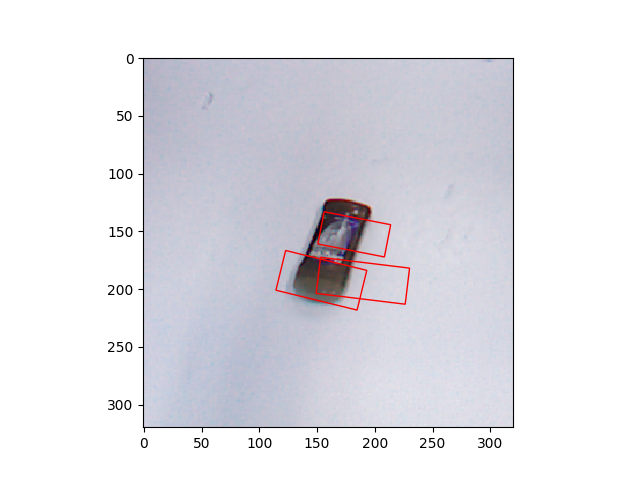
\includegraphics[width=0.4\textwidth]{figures/rgrasp_prediction_good.png}}
\qquad
\subfloat{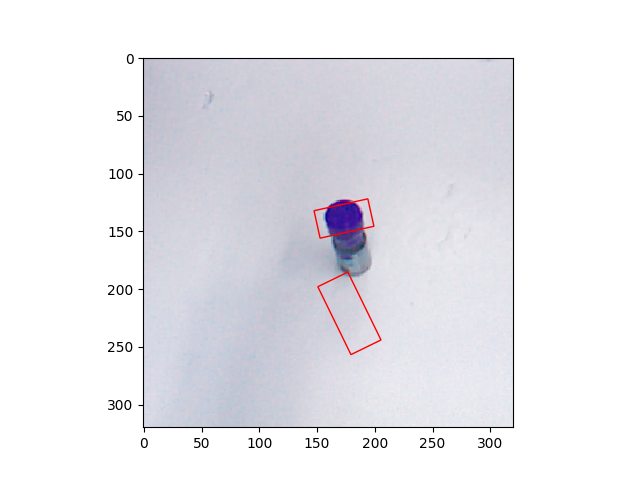
\includegraphics[width=0.4\textwidth]{figures/rgrasp_prediction_2.png}}
\qquad
\subfloat{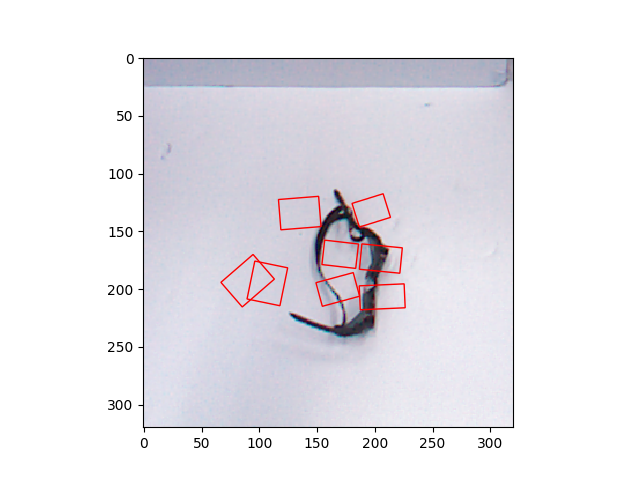
\includegraphics[width=0.4\textwidth]{figures/rgrasp_prediction_3.png}}
\qquad
\subfloat{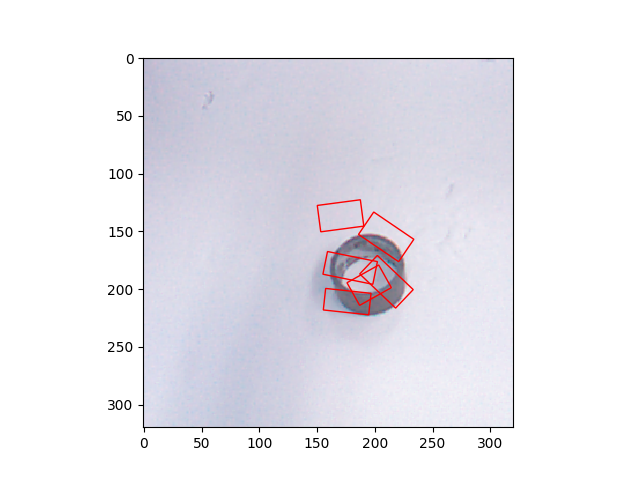
\includegraphics[width=0.4\textwidth]{figures/rgrasp_prediction_4.png}}
\caption{examples of inference done by the model}
\label{fig:rgrasp_examples}
\end{figure}

\begin{figure}
\centering
\subfloat[Train]{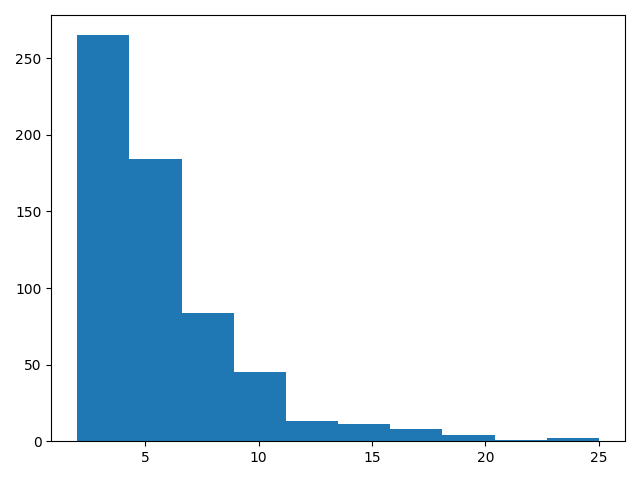
\includegraphics[width=0.4\textwidth]{figures/trainrecdist.png}}
\qquad
\subfloat[Val]{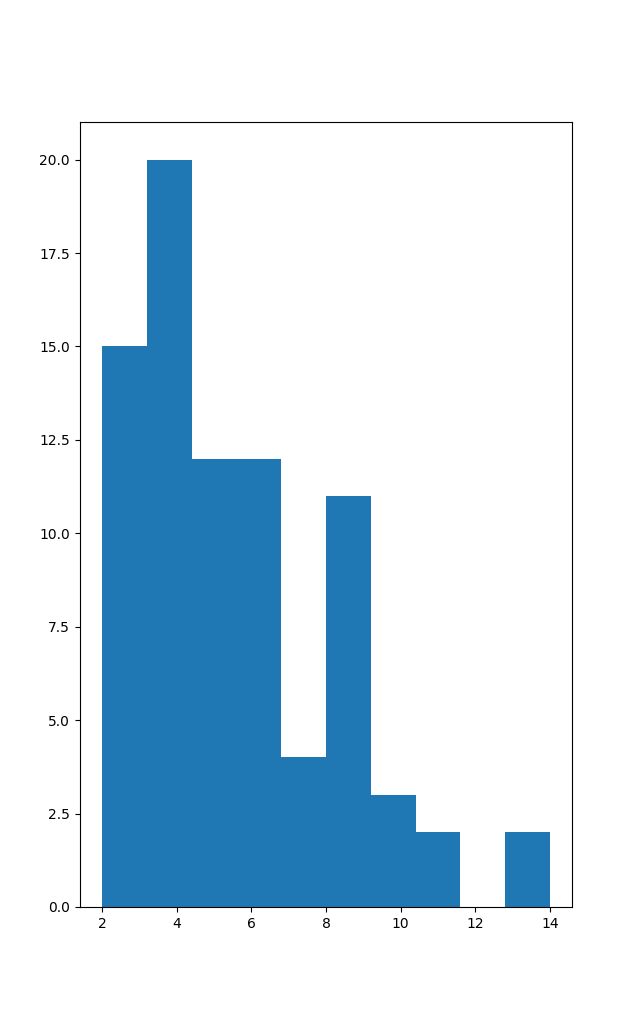
\includegraphics[width=0.4\textwidth]{figures/valrecdist.png}}
\caption{The Distribution of Rectangles per Image on the Training and Validation Sets}
\label{fig:recdist}
\end{figure}

\begin{figure}
\centering
\subfloat[Cross Entropy]{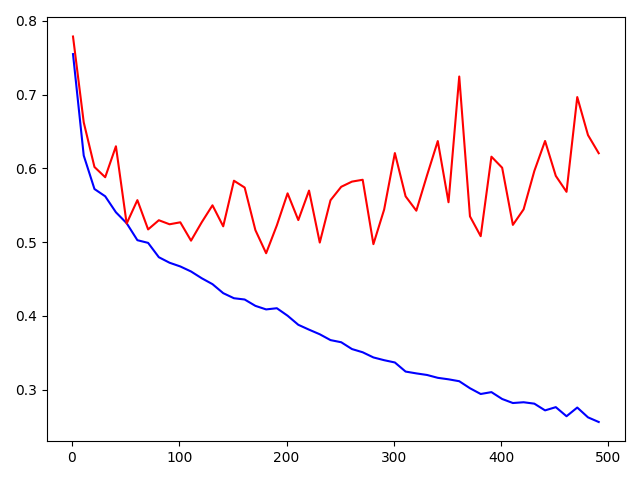
\includegraphics[width=0.4\textwidth]{figures/rgrasp_detection_loss.png}}
\qquad
\subfloat[Smooth L1 Loss]{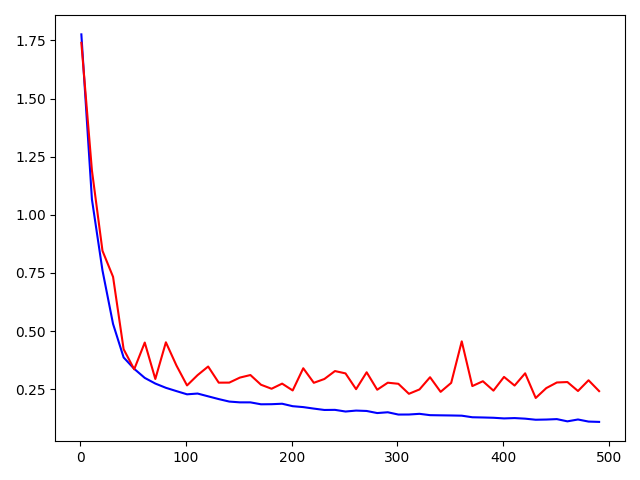
\includegraphics[width=0.4\textwidth]{figures/rgrasp_regression_loss.png}}
\caption{Loss Values over 500 Epochs of training. Training Loss (Red) and Validation Loss (Blue)}
\label{fig:rgrasp_loss}
\end{figure}

\begin{figure}
\centering
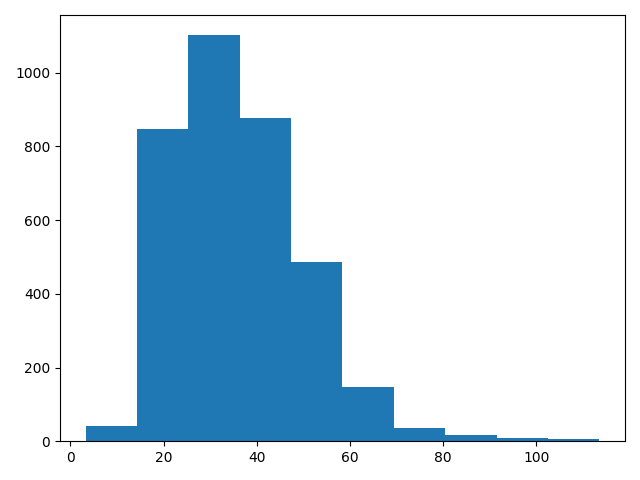
\includegraphics[width=0.4\textwidth]{figures/bbox_area_dist_train.png}
\caption{Distribution of bounding box areas}
\label{fig:areas}
\end{figure}


\bibliographystyle{plain}
\bibliography{bibliography.bib}

\end{document}
